% Overleaf: paste into main.tex and compile with pdfLaTeX.
% Self-contained: no external figures or bibliography file required.
\documentclass[11pt,a4paper]{article}
\usepackage[margin=2.3cm]{geometry}
\usepackage[T1]{fontenc}
\usepackage[utf8]{inputenc}
\usepackage{lmodern}
\usepackage{microtype}
\usepackage{amsmath,amssymb,booktabs,tabularx}
\usepackage{tikz}
\usetikzlibrary{positioning,arrows.meta}
\usepackage[colorlinks=true,linkcolor=blue!50!black,urlcolor=blue!60!black]{hyperref}
\newcommand{\file}[1]{\nolinkurl{#1}}
\setlength{\parindent}{0pt}
\setlength{\parskip}{5pt}
\setlength{\emergencystretch}{2em}
\renewcommand{\arraystretch}{1.15}
\title{From Semantic Induction Heads to Multi-hop Circuits\\
\large Research Progress and Experiment Record}
\author{Daniella Simonovsky and Max Golubkov}
\date{Working record based on the available project files}

\begin{document}
\maketitle

\section{Scope and Current Status}
This document records the project from the initial proposal to the latest available behavioral experiments. It explains the main decisions, results, and remaining work. It is a research log, not a final paper.

\textbf{Completed:} literature study, methodology design, model selection, synthetic data generation, evaluation infrastructure, and behavioral pilots with Pythia-1B and Pythia-6.9B.

\textbf{Not yet completed:} Relation Index (RI) measurements on our models, activation or path patching, circuit extraction, faithfulness evaluation, or analysis across training checkpoints. We have not yet identified a Semantic Induction Circuit (SIC).

The record uses the proposal, project discussions, code, saved reports, and result files. Later completion-v3 and v3.1 runs were found in the project directory and are included below. Stages are ordered by experiment version; comments and random seeds in code are not treated as verified execution dates.

\section{Initial Proposal}
The proposal, \emph{From Heads to Circuits: Identifying Semantic Induction Circuits for Multi-hop Reasoning in LLMs}, asked:
\begin{quote}
How do language models process multi-hop semantic relations? Are these relations handled by individual semantic induction heads or by distributed circuits across layers?
\end{quote}
Our initial example was transitive inclusion:
\[
A\subseteq B,\qquad B\subseteq C \quad\Rightarrow\quad A\subseteq C.
\]
Retrieving $A\subseteq B$ is a one-hop control. It does not itself require transitive inference.

The proposal suggested open model suites such as Pythia, OLMo, or LMEnt; activation and path patching; an extension of RI from heads to circuits; and faithfulness tests on a sparse subgraph. Public training checkpoints would support a later study of circuit development. Synthetic tasks inspired by bAbI and CLUTRR were considered, but no evaluation on those original datasets is documented here.

We made behavioral validation the first practical step: before explaining a mechanism, we needed a model that reliably performed the target task.

\section{Literature and Methodological Foundations}
\subsection{Core Reading}
We studied three central sources:
\begin{itemize}
\item \textbf{A Mathematical Framework for Transformer Circuits} \cite{framework}: the residual stream, QK and OV computations, and composition through queries, keys, and values.
\item \textbf{In-context Learning and Induction Heads} \cite{olsson}: the classical pattern $\ldots,A,B,\ldots,A\rightarrow B$. In the simple two-layer mechanism, an earlier previous-token head supports a later induction head. The head and the full circuit are distinct objects.
\item \textbf{Identifying Semantic Induction Heads to Understand In-Context Learning} \cite{ren}: attention-head behavior associated with semantic or syntactic relations, measured using RI. This was the direct starting point for our research question.
\end{itemize}

We distinguished semantic-head diagnostics from classical induction tests. Calling a head an SIH does not establish that it implements the classical copying circuit. We therefore planned separate prefix-matching and copying controls.

We also distinguished the reference paper's tasks from ours. Relation analysis in natural text and its ICL evaluations are not equivalent to composing new facts about invented entities. Its reported performance is therefore not a directly comparable baseline for our synthetic task.

\subsection{Additional Sources}
We reviewed additional approaches and collected supporting papers on:
\begin{itemize}
\item circuit analysis and path patching, including the indirect-object identification circuit \cite{ioi};
\item activation-patching methods and measurement choices \cite{patchguide};
\item automated circuit discovery, position-aware analysis, and faithfulness;
\item feed-forward layers as key-value memories and feature superposition;
\item induction-head development and learning dynamics.
\end{itemize}
The depth of study differed across papers. A paper's presence in our library does not mean we reproduced it. These sources also motivated alternatives to a heads-only explanation, including MLP contributions and distributed representations.

\section{Planned Mechanistic Analysis}
We designed several complementary lines of evidence. They are not assumed to be statistically independent.

\begin{enumerate}
\item \textbf{Behavioral controls.} Test direct relations, two-hop composition, changed facts, and robustness before interpreting internal components.
\item \textbf{Candidate-head diagnostics.} Use RI, attention patterns, and local output projections to identify components worth testing. Include random-head and random-target controls. RI is observational evidence, not proof that a head is necessary for the answer.
\item \textbf{Node interventions.} Use activation patching and ablation to measure the effect of changing a component's activation. These are causal interventions within the model, but their interpretation depends on the replacement values, inputs, and outcome metric.
\item \textbf{Directed connections.} Use path patching to test whether an earlier component affects the output through a later one. Separate effects on Q/K from effects on V. Two individually important heads are not sufficient evidence of a shared circuit.
\item \textbf{Circuit validation.} Test a proposed sparse circuit for recovery of model behavior, sensitivity to removal, and generalization to new examples. Specify the ablation baseline and recovery criterion in advance.
\end{enumerate}

We discussed a conditional circuit score: whether a later head's relation-related activity depends on an earlier head's activity. This remains a proposal, not an implemented or validated metric. Correlated or multiplied RI scores alone would not establish information flow.

A possible intervention outcome is the answer margin
\[
m(x)=\log P(y_{\mathrm{target}}\mid x)-\log P(y_{\mathrm{alternative}}\mid x).
\]
Patching can then be evaluated by the change in this margin. The target must remain fixed when comparing clean and changed inputs. Normalized recovery scores require care when the clean--changed difference is small.

\begin{figure}[ht]
\centering
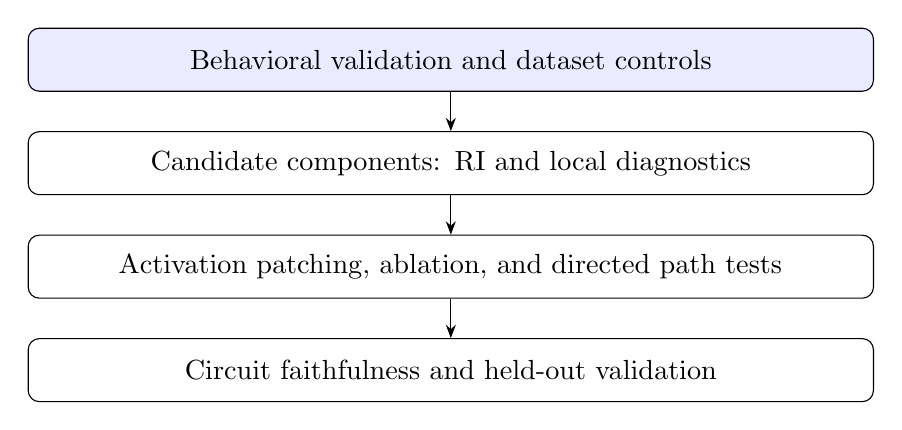
\begin{tikzpicture}[node distance=5mm,>=Stealth,
box/.style={draw,rounded corners,align=center,text width=10.5cm,minimum height=8mm}]
\node[box,fill=blue!8] (a) {Behavioral validation and dataset controls};
\node[box,below=of a] (b) {Candidate components: RI and local diagnostics};
\node[box,below=of b] (c) {Activation patching, ablation, and directed path tests};
\node[box,below=of c] (d) {Circuit faithfulness and held-out validation};
\draw[->] (a)--(b); \draw[->] (b)--(c); \draw[->] (c)--(d);
\end{tikzpicture}
\caption{Planned workflow. Work to date focuses on the first stage and evaluation infrastructure.}
\end{figure}

\section{Models, Data, and Infrastructure}
\subsection{Model and Resource Decisions}
We started with Pythia-1B because it was small enough for an initial pilot and belonged to an open model suite with training checkpoints. After weak behavioral results, we moved to Pythia-6.9B within the same family. OLMo and InternLM alternatives were discussed but are not documented as evaluated models.

Both models were used as English base language models. ICL examples were added to the prompt; model weights were not updated. No pretraining or fine-tuning was performed. The pinned revisions were:
\begin{itemize}
\item Pythia-1B: \file{f73d7dcc545c8bd326d8559c8ef84ffe92fea6b2}.
\item Pythia-6.9B: \file{c0e3eee36dc47af0c49f361c74cfe459c09f7f23}.
\end{itemize}

The project had access to TAU Slurm GPUs and storage, with roughly three weeks remaining when resource planning was discussed. We prepared for portability to Colab or RunPod, but the documented results came from the cluster workflow. Some 6.9B runs used model sharding across two 11GB RTX 2080 Ti GPUs; this should not be assumed for every later run.

\subsection{Data Design}
Early datasets were generated as graphs before conversion to text. We stored facts, queries, gold answers, proof paths, entity spans, family IDs, variants, and seeds. This supported checks of reachability and required path length.

The four checks were:
\begin{enumerate}
\item direct relation retrieval;
\item two-hop composition;
\item a changed fact that breaks or redirects the relevant chain;
\item robustness to fact order, distractors, and renamed entities.
\end{enumerate}
Invented names reduced reliance on memorized facts about specific entities. They did not eliminate prior knowledge of language or relations, and could introduce tokenization difficulty.

\subsection{Execution and Debugging}
We implemented data generators, Slurm submission, multi-GPU execution, smoke tests, resumable runs, result merging, and analysis scripts. Manifests and file hashes recorded model and dataset identity. Work was partitioned by complete families to keep related examples together.

Early runs encountered environment, loading, and numerical failures. Non-finite scores in the larger model led to a working SDPA MATH configuration with FP16 weights and explicit finite-value checks. This resolved the observed execution failures without proving which operation first caused the numerical issue. FP32 spot checks and careful tie handling were discussed; a full FP32 rerun is not documented.

Tokenization was treated explicitly: names can span several tokens, and candidate scores must cover the full completion. Saved outputs allowed inspection of exact prompts, generated tokens, answer scores, and entity locations.

\section{Evaluation Measures}
\textbf{Free accuracy} measures whether the name extracted from unrestricted generation equals the gold answer. \textbf{Candidate accuracy} measures whether the correct answer receives the higher score among two specified names:
\[
s(y\mid x)=\sum_{i=1}^{k}\log P(t_i\mid x,t_{<i}),
\]
where the scored continuation includes the leading space and final period according to the tokenizer. A mean score per token was also saved as a diagnostic.

Greedy generation and full-sequence ranking can disagree. A 50\% random baseline applies to balanced two-candidate selection, not unrestricted generation. Early completion prompts displayed the candidates; later natural-language prompts did not.

We also examined label bias, format compliance, ties, intermediate-entity answers, position effects, and success on both members of a control pair. Confidence intervals must account for related examples within families rather than treating all prompts as independent.

\section{Experiment History}
\subsection{Pythia-1B: Yes/No Pilot}
The initial task used names such as \texttt{group000a}, graph-derived labels, and four fixed demonstrations. A zero-shot dataset was also prepared; the full run summarized here used four shots. ``No'' meant that the query was not entailed, not that its opposite was proved.

Across 1,200 prompts, free accuracy was 53.5\% for direct relations and 61.0\% for two-hop queries. The model strongly favored Yes: direct positive accuracy was 88\%, compared with 19\% on negatives. Breaking the first or second link yielded only 20\% and 17\% free accuracy. These results did not justify circuit analysis.

We decided to try a larger model, more distinct names, and more demonstrations. Name similarity was a possible difficulty, not an established cause.

\subsection{Pythia-6.9B: Yes/No and Demonstration Revisions}
We replaced similar labels with names such as \texttt{wugs} and \texttt{daxes}, and ran 4- and 12-shot conditions. In the first completed 4-shot run, every free answer was No. In the 12-shot run, 1,154 of 1,200 free answers were No.

The dataset contained 700 No and 500 Yes labels. Always answering No therefore achieved 58.33\% overall and 100\% on the all-negative broken-chain subset. Overall accuracy was misleading.

We then varied demonstrations across families, balanced labels and final labels, and improved structural matching. This Yes/No revision was called \texttt{prompt-v3}; it is distinct from the later \texttt{completion-v3}. The revised 4-shot model still answered No everywhere. With 12 shots, it produced 1,194 No answers and six Yes answers. Direct and two-hop accuracy remained 50\%. Copying the final demonstration label alone did not explain the behavior.

\subsection{Completion-v1: Answering with a Name}
We replaced Yes/No with name completion, using 1,200 questions in each of the 0-, 4-, and 12-shot conditions. Two candidates were shown. For two-hop questions, the intermediate entity was excluded from the candidate pair.

\begin{center}\small
\begin{tabular}{lrrr}
\toprule
Check & 0 shots & 4 shots & 12 shots\\\midrule
Direct & 56.0 / 70.5 & 79.5 / 91.0 & 77.0 / 88.5\\
Two-hop & 17.5 / 50.0 & 28.0 / 71.5 & 35.0 / 75.0\\
Redirected chain & 22.5 / 58.0 & 20.0 / 59.0 & 26.5 / 55.0\\
Robustness & 18.2 / 55.5 & 20.8 / 67.0 & 29.7 / 65.0\\\bottomrule
\end{tabular}
\end{center}
\textit{All result tables report free / candidate accuracy in percent. Each condition contains 200 direct, 200 two-hop, 200 changed-chain, and 600 robustness prompts.}

Two important problems emerged:
\begin{itemize}
\item \textbf{Intermediate answers.} With 12 shots, 100 of 200 two-hop outputs named the intermediate entity, 70 named the target, and 30 named the wrong candidate. In $A\rightarrow B\rightarrow C$, completing ``All A are'' with B is logically valid, although it ignores the candidate restriction.
\item \textbf{Frequency shortcut.} Both candidates appeared in the facts, but the correct candidate often appeared more frequently. Choosing the more frequent candidate, with random tie-breaking, achieved an expected 83.3\% overall and 100\% on basic two-hop questions.
\end{itemize}
We also observed candidate-position preferences. These findings establish weaknesses in the test, not proof that the model used frequency or position as its mechanism.

For example, a prompt contained \texttt{vromps}\,$\rightarrow$\,\texttt{ruspins}\,$\rightarrow$\,\texttt{kelbrins}, plus facts mentioning \texttt{kelbrins} twice and \texttt{snorps} once. The model correctly answered \texttt{kelbrins}. After changing the chain to \texttt{vromps}\,$\rightarrow$\,\texttt{tivaks}\,$\rightarrow$\,\texttt{snorps}, it still answered \texttt{kelbrins}. This is consistent with several shortcuts and does not distinguish them.

With 12 shots, free success on both the original and changed question was only 3\% for first-link changes and 13\% for second-link changes; candidate success was 19\% and 45\%. Pair success is different from accuracy on the changed question alone.

\subsection{Completion-v2: Explicit Depth and Balanced Controls}
We made the task explicit: identify the group whose shortest chain from the source has exactly one or two steps. The same wording appeared in demonstrations. The target was unique at the requested depth even without the candidate list.

We balanced candidate mentions and subject/object roles, added reversed candidate-order pairs, and changed two facts when redirecting the chain so that entity counts remained fixed. Each condition contained 50 families $\times$ 12 questions $\times$ two option orders: 1,200 prompts representing 600 content questions.

Construction checks passed. The frequency baseline became 50\%; simple fact-position baselines were approximately 48--53\% across the main checks. Available full-run results were:
\begin{center}\small
\begin{tabular}{lrr}
\toprule
Check & 4 shots & 12 shots\\\midrule
Direct & 50.5 / 50.5 & 56.0 / 56.0\\
Two-hop & 49.0 / 49.5 & 52.0 / 52.0\\
Redirected chain & 51.5 / 53.0 & 46.5 / 46.5\\
Robustness & 47.7 / 48.0 & 50.2 / 50.2\\\bottomrule
\end{tabular}
\end{center}
The revision did not establish reliable task performance. Format sensitivity is a plausible explanation, but wording and dataset structure changed together, so wording alone was not isolated as the cause. The version was retained as a negative result. A zero-shot dataset was prepared, but no full result for it was found in this review.

\subsection{Completion-v3: Natural Language and Named Composed Relations}
Later files introduced natural-language questions without an instruction preamble or visible options. Kinship was the anchor task: mother and grandmother provide distinct names for the direct and composed relations. Motherhood itself is not transitive; two mother links compose into a grandmother relation.

The dataset also included containment and location. Intermediate answers remain potentially valid in their free-completion formats and require separate treatment. The 100 families comprised 68 kinship, 16 containment, and 16 location families. Each had six questions and two fact-order variants, giving 1,200 prompts per shot condition.

Candidate mentions were balanced and candidate token lengths matched. Forty separate retrieval and verbatim-demonstration controls were prepared; their execution results were not found in this review. Failure on such controls would require diagnosis, not automatically prove a software bug.

\begin{center}\small
\begin{tabular}{lrr}
\toprule
Check & 4 shots & 12 shots\\\midrule
Direct & 84.0 / 86.5 & 85.5 / 87.0\\
Two-hop & 61.0 / 71.0 & 59.5 / 67.0\\
Redirected chain & 40.0 / 46.0 & 46.5 / 50.5\\
Robustness & 42.7 / 60.2 & 45.3 / 63.5\\\bottomrule
\end{tabular}
\end{center}

\subsection{Completion-v3.1: Crossing Depth and Order in Demonstrations}
Code comparison showed that the first v3 demonstration bank coupled hop count with fact-block order. Version v3.1 crossed the two factors and sampled equally from the four combinations.

\begin{center}\small
\begin{tabular}{lrrr}
\toprule
Check & 0 shots & 4 shots & 12 shots\\\midrule
Direct & 23.5 / 71.5 & 87.0 / 90.0 & 88.0 / 89.5\\
Two-hop & 18.5 / 63.5 & 62.5 / 78.5 & 64.5 / 79.0\\
Redirected chain & 11.5 / 51.0 & 39.5 / 49.5 & 41.5 / 49.5\\
Robustness & 10.8 / 55.3 & 46.3 / 68.2 & 47.2 / 68.0\\\bottomrule
\end{tabular}
\end{center}
For kinship alone with 12 shots, candidate accuracy was 91.9\% on direct questions, 86.0\% on two-hop questions, and 46.3\% on redirected chains. The basic task signal improved, but changed-fact performance remained weak. Regenerating demonstrations can also change sampled names and examples; differences between versions are not isolated effects of one change.

\section{Known Limitations and Audit Status}
Earlier completion-v1 results received a detailed audit of coverage, tokenization, scoring, and graph labels. For later versions, the figures above were recomputed from saved correctness fields and 1,200 unique IDs were checked per run. This was not a full revalidation of every token score or gold label.

The documentation review identified additional issues in v3/v3.1:
\begin{itemize}
\item \textbf{Broken base links:} 800 \texttt{paired\_base\_id} references per run omit the order suffix and do not match result IDs. The inspected paired-metric files are empty; this means the analysis was not produced, not that pair accuracy was zero.
\item \textbf{Changed demonstrations within pairs:} in 4- and 12-shot runs, the two fact-order variants also receive different demonstrations. Their difference does not isolate fact order.
\item \textbf{Legacy field names:} \texttt{option\_order} now denotes fact order, although no candidate options appear in the prompt.
\item \textbf{Renaming and reproducibility:} semantic comparison requires an explicit name mapping. The later generator also uses Python's \texttt{hash()} for distractor placement; reproducibility requires controlling this source of randomness or preserving the exact generated files.
\end{itemize}
These issues were recorded, not repaired as part of writing this document. Historical results were not modified.

\section{Main Lessons and Next Steps}
\begin{enumerate}
\item \textbf{Validate the task before interpreting the model.} Correct graph labels do not rule out shortcuts, ambiguity, or demonstration leakage.
\item \textbf{Separate accuracy from robustness.} Strong basic two-hop accuracy is insufficient when answers fail to track changed facts.
\item \textbf{Keep comparisons controlled.} Model size, prompt format, names, demonstrations, and graph structure changed across stages. Their individual effects cannot be inferred from aggregate differences.
\item \textbf{Use multiple forms of evidence.} RI can identify candidates; interventions test effects; directed-path and circuit-level tests support stronger mechanistic claims.
\end{enumerate}

Next, repair pair construction and analysis, run the prepared controls, and select a clear anchor task. Freeze development and held-out families before further prompt tuning. Define a behavioral entry criterion in advance, including changed-fact and paired robustness tests. Only then proceed to component screening and targeted interventions.

The current outcome is an evaluation pipeline, a documented sequence of task revisions, and evidence of important limitations. It is not yet evidence of an identified SIH or SIC. A different mechanism, a narrower research question, or a model change remain valid outcomes.

\appendix
\section{Source Files}
Paths are relative to \texttt{final proj/project}. Preserve raw prompts and results in addition to summaries.
\begin{itemize}
\item Proposal: \file{../NLP Projects_Proposal.pdf}; papers: \file{../papers/}.
\item Initial plan: \file{data_pipeline_plan.tex}.
\item 1B pilot: \file{pythia_pilot/}; results: \file{results/full_4shot_review/storage/runs/full_4shot/}.
\item 6.9B Yes/No: \file{results/full_sdpa_review/} and \file{results/prompt_v3_review/}.
\item Completion-v1: \file{results/completion_review/}; detailed audit: \file{results/completion_analysis/}.
\item Completion-v2: \file{pilot_v2/build_completion_v2_data.py}; results: \file{results/completion_v2_4shot_v1/} and \file{results/completion_v2_12shot_v1/}.
\item Later generators: \file{pilot_v3/build_data_v3.py} and \file{pilot_v3/upload/build_data_v3.py}.
\item Later results: \file{results/completion_v3_4shot_v1/}, \file{results/completion_v3_12shot_v1/}, and \file{results/completion_v3_1_0shot/}, \file{results/completion_v3_1_4shot/}, \file{results/completion_v3_1_12shot/}.
\end{itemize}

\begin{thebibliography}{9}
\bibitem{ren} Jie Ren et al. (2024). \emph{Identifying Semantic Induction Heads to Understand In-Context Learning}. Findings of ACL, 6916--6932. \url{https://aclanthology.org/2024.findings-acl.412/}
\bibitem{olsson} Catherine Olsson et al. (2022). \emph{In-context Learning and Induction Heads}. Transformer Circuits Thread. \url{https://transformer-circuits.pub/2022/in-context-learning-and-induction-heads/index.html}
\bibitem{framework} Nelson Elhage et al. (2021). \emph{A Mathematical Framework for Transformer Circuits}. Transformer Circuits Thread. \url{https://transformer-circuits.pub/2021/framework/index.html}
\bibitem{ioi} Kevin Wang et al. (2022). \emph{Interpretability in the Wild: a Circuit for Indirect Object Identification in GPT-2 Small}. \url{https://arxiv.org/abs/2211.00593}
\bibitem{patchguide} Stefan Heimersheim and Neel Nanda (2024). \emph{How to Use and Interpret Activation Patching}. \url{https://arxiv.org/abs/2404.15255}
\end{thebibliography}
\end{document}
